\section{Results and Discussion}
System-level simulation was performed with representative AI inference workloads.

\subsection{Standby Power}
Migrating cold data and checkpoints to the FeRAM-backed tier yields more than 30\% reduction in standby power.
This reduction arises from suppressing periodic DRAM refresh for inactive regions.

\subsection{Resume Latency}
FeRAM allows direct restore of checkpoints without full DRAM wake-up.
Resume latency is reduced to the $\mu$s range, enabling near-instant resume after power gating and improving energy efficiency for mobile edge AI.

\subsection{Endurance}
FeRAM endurance of $10^{12}$~writes/year fits within FeRAM capability for checkpoint traffic.

% ==== Fig.2: Access time vs retention(x:10^0-10^2 ns, y:10^0-10^4 s)====
\begin{figure}[!t]
\centering
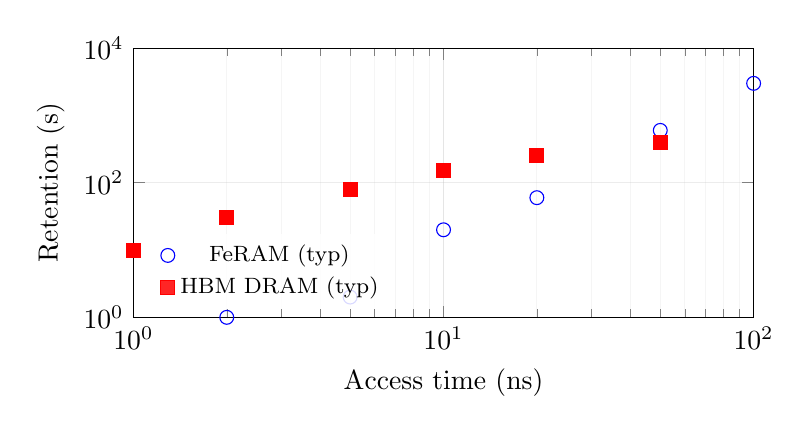
\begin{tikzpicture}
\begin{axis}[
  width=0.78\linewidth, height=5.0cm,
  xmode=log, ymode=log,
  xmin=1e0, xmax=1e2, ymin=1e0, ymax=1e4,
  xlabel={Access time (ns)}, ylabel={Retention (s)},
  tick align=inside,            % ← 目盛りを内側へ
  grid=both,
  minor grid style={opacity=0.15},
  major grid style={opacity=0.30},
  legend style={
    draw=none, fill=white, fill opacity=0.85, text opacity=1,
    at={(0.03,0.03)}, anchor=south west, font=\footnotesize
  },
  mark size=2.5pt
]
  % FeRAM(青○)
  \addplot[only marks, mark=o, blue]
    coordinates {(2,1) (5,2) (10,20) (20,60) (50,600) (100,3000)};
  % HBM DRAM(赤■)
  \addplot[only marks, mark=square*, red]
    coordinates {(1,10) (2,30) (5,80) (10,150) (20,250) (50,400)};
  \legend{FeRAM (typ), HBM DRAM (typ)}
\end{axis}
\end{tikzpicture}
\caption{Access time vs.\ retention. 赤■: HBM、青○: FeRAM。目盛りは\emph{内向き}。%
表示範囲は $10^0\!\sim\!10^2$ ns, $10^0\!\sim\!10^4$ s。}
\label{fig:access_retention}
\end{figure}
